\subsection{Gestione magazzini: Jolie}
L'implementazione della gestione dei magazzini \`e stata fatta
utilizzando una SOA di servizi Jolie. I file utilizzati sono quelli
contenuti nella directory \linebreak {\tt Magazzini}.
La gestione del magazzino viene dunque implementata utilizzando tre
componenti principali: 
\begin{itemize}
  \item magazzino primario, suddiviso in:
    \begin{itemize}
      \item interfaccia ({\tt interfMagazzinoPrimario.iol});
      \item implementazione ({\tt magazzinoPrimario.ol});
    \end{itemize}
  \item magazzini secondari, suddivisi in:
    \begin{itemize}
      \item interfaccia ({\tt interfMagazzinoSecondario.iol});
      \item implementazione ({\tt magazzinoSecondarioX.iol});
    \end{itemize}
  \item tipi di dato utili alle operazioni ({\tt dataTypes.iol});
  \item un database relazionale implementato dal DBMS HSQL (la libreria
  \`e contenuta nella directory {\tt lib}).
\end{itemize}
Il database implementato, pur essendo elementare, contiene tutte le
entit\`a necessarie per una buona approssimazione di un database reale:
abbiamo dunque la tabella {\tt pezzo}, la tabella {\tt magazzino} e la
tabella {\tt pezzo\_magazzino}, che implementa una relazione tra le
prime due tabelle.

\subsubsection*{\tt intefacciaMagazzinoPrimario.iol}
Interfaccia che contiene le operazioni che possono essere effettuate dal
magazzino primario. Le operazioni sono tutte del tipo
{\tt RequestResponse}, come mostrato in figura. \\\\
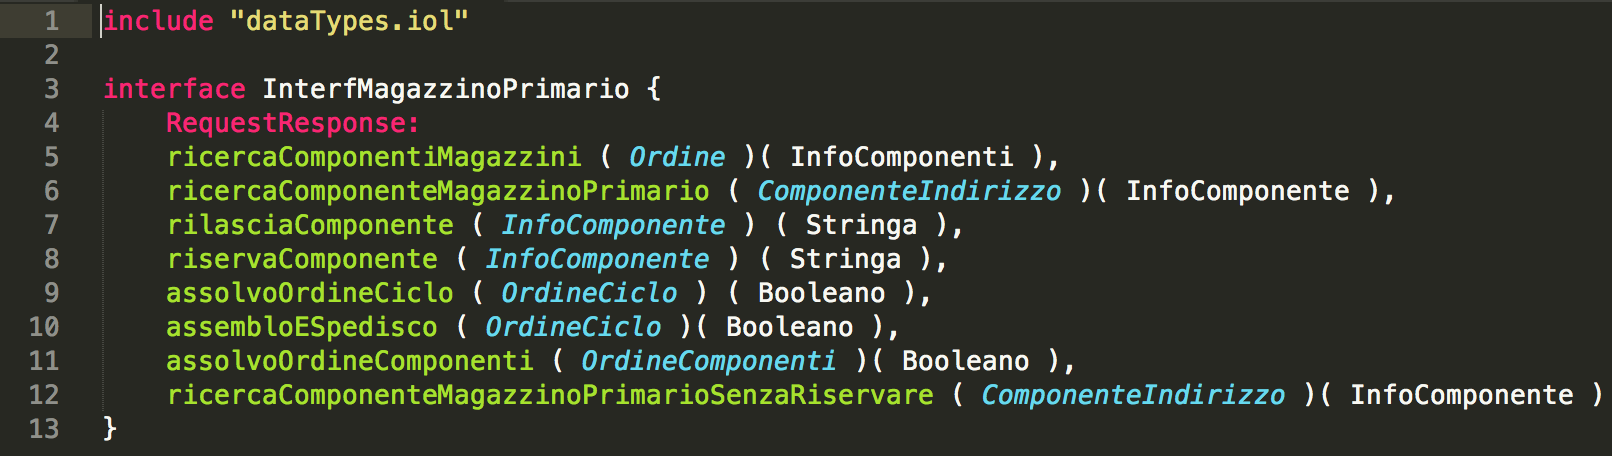
\includegraphics[scale=0.4]{immagini/interfMagazzinoPrimario.png}

\subsubsection*{\tt magazzinoPrimario.ol}
Questo file contiene l'implementazione delle operazioni del magazzino
primario. Contiene una {\tt inputPort}, in ascolto sulla porta {\tt 8000}
utilizzando un protocollo {\tt soap}, ed una serie di {\tt outputPort},
per gestire le interazioni con:
\begin{itemize}
  \item se stesso ({\tt soap}, {\tt 8000});
  \item il primo magazzino secondario ({\tt soap}, {\tt 8001});
  \item il secondo magazzino secondario ({\tt soap}, {\tt 8002});
  \item il servizio di calcolo delle distanze ({\tt http}, {\tt 8100});
  \item il servizio del fornitore ({\tt http}, {\tt 8300});
  \item il servizio di corriere ({\tt http}, {\tt 8400}).
\end{itemize}
Viene poi creata una procedura {\tt leggiImpostazioni}, nella quale
vengono prese le configurazioni del database necessarie al magazzino
primario dal file {\tt magazzinoPrimario.conf}. Tali impostazioni
vengono poi utilizzate nella procedura di connessione al database,
{\tt connettiDB}. Un'altra procedura implementata \`e quella di chiusura
della connessione con il database, {\tt disconettiDB}.

Si incontra poi la procedura {\tt inizializzaInfoMagazzini} che, prese
le informazioni dal database, inserisce nell'array dei magazzini le
corrette informazioni.

Viene poi implementata una procedura di {\tt init}, che lancia le
procedure elencate in precedenza e setta correttamente le variabili
{\tt magazzinoPrimario} e {\tt officina}.

Vengono poi implementate le operazioni definite nell'interfaccia:
\begin{itemize}
  \item {\tt verificaDisponibilitaERiservaPezzi}: i pezzi presi
  dall'ordine vengono cercati uno per uno all'interno del sistema: se
  qualcuno di essi risulta non disponibile, viene richiesto al fornitore
  di riservarcene la quantit\`a richiesta (senza per\`o ordinargliela).
  \item {\tt verificaDisponibilitaPezziNelDBERiservaDisponibili}:
  operazione utilizzata da quella precedente per verificare tramite il
  database la presenza di un pezzo. Se esso \`e presente, viene
  riservato. In questa operazione si pu\`o osservare il seguente
  meccanismo: il pezzo viene riservato nel magazzino pi\`u vicino al
  cliente, se esso pu\`o essere spedito singolarmente; altrimenti viene
  riservato nel magazzino pi\`u vicino all'officina;
  \item {\tt annulloOrdine}: operazione per annullare correttamente
  l'ordine, cancellando la riserva dai pezzi, azzerando diversi valori
  utili alla spedizione, \dots re-impostando dunque il sistema allo
  stesso stato che aveva prima dell'ordine;
  \item {\tt eseguoOrdine}: questa operazione si occupa della
  preparazione dei vari pezzi all'ordine, preparandolo alla spedizione
  al cliente o all'officina;
  \item {\tt assemblaCicloESpedisci}: assolve virtualmente al compito
  di assemblare il ciclo per il cliente e di spedirlo;
  \item {\tt spedisciDaMagazzini}: si occupa della spedizione di un
  pezzo atomico dal magazzino pi\`u vicino al cliente;
  \item {\tt richiestaSpedizione}: si occupa di richiedere la spedizione
  al fornitore.
\end{itemize}

\subsubsection*{\tt intefacciaMagazzinoSecondario.iol}
Interfaccia che contiene l'operazione che effettuano i magazzini
secondari. Questa interfaccia \`e comune a tutti i magazzini secondari.
L'operazione \`e del tipo {\tt RequestResponse}, come mostrato in
igura. \\\\
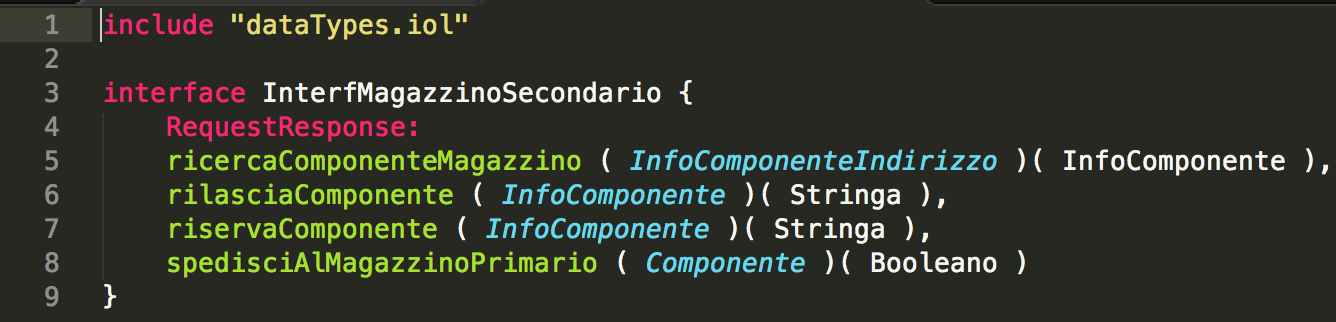
\includegraphics[scale=0.5]{immagini/interfMagazzinoSecondario.png}

% old

\subsubsection*{\tt magazzinoSecondario[x].ol}
Mentre il file di interfaccia dei magazzini secondari \`e unico per
tutti, le implementazioni sono tante quanti sono i magazzini secondari.

Come si pu\`o intuire, utilizzando questo meccanismo, aggiungere o
cancellare un magazzino secondario diventa un'operazione estremamente
semplice: basta aggiungere/eliminare il file
{\tt magazzinoSecondario[x].ol} corrispondente ed aggiungere/eliminare
le informazioni e l'{\tt OutputPort} all'interno del file di
implementazione del magazzino primario.
Contiene una {\tt inputPort}, in ascolto sulla porta {\tt 800[x]} con
protocollo {\tt soap}, ed una {\tt outputPort} per interagire con il
servizio di calcolo delle distanze ({\tt http}, {\tt 8100}).
Non sono contemplate interazioni con altri magazzini secondari, poich\'e
la coordinazione viene completamente gestita dal magazzino primario.

Viene poi implementata l'unica operazione dell'interfaccia, cio\`e
{\tt richiestaSpedizione}, che si occupa di richiedere la spedizione di
un pezzo riservato al cliente. Il magazzino secondario \`e stato
estremamente semplificato, in quanto si `e preferito lasciare la maggior
parte della gestione al magazzino primario.

\subsubsection*{\tt dataTypes.iol}
Questo file contiene i tipi di dato che verranno utilizzati all'interno
della soluzione.

\subsubsection*{\tt creaDBmagazzinoPrimario.ol}
Questo file contiene tutte le istruzioni necessarie all'inizializzazione
del database. Innanzitutto dunque andrà a fissare i parametri di
connessione, come per esempio username, password, porta di connessione,
\dots \\
Inizializzati i parametri, vengono eseguite le istruzioni necessarie per
la creazione delle tabelle del database.

\subsubsection*{\tt insertDB.ol}
Contiene le istruzioni necessarie per inserire all'interno del database
un insieme di oggetti di esempio, per poter mostrare fin dal primo avvio
le funzionalit\`a del sistema.

